% !TEX program = xelatex
% ¡Recuerda compilar con XeLaTeX o LuaLaTeX!
\documentclass{article}

% --- Cargar nuestro fichero de estilo ---
% Se asume que paper_style.sty está disponible o se usan paquetes estándar.
\usepackage{paper_style}

% --- PAQUETES PARA EL CONTENIDO DEL DOCUMENTO ---
\usepackage{graphicx}
\usepackage{subcaption}
\usepackage{amsmath}
\usepackage{booktabs}
\usepackage{geometry}
\usepackage{hyperref}
\usepackage{enumitem}
\usepackage{float}


% --- Información del Paper ---
\title{Práctica 1: Experimentación con Graph Neural Networks}
\author{
	Jordi Blasco Lozano \\
	\small Universidad de Alicante \\
	\small Agentes Inteligentes
}
\date{\today}

% --- Comienzo del Documento ---
\begin{document}
	
	\maketitle

	\begin{abstract}
	\noindent Este informe presenta una experimentación exhaustiva con Graph Neural Networks (GNNs) para tareas de clasificación de nodos. Se crea un dataset sintético custom con 2000 nodos y se compara el rendimiento de Multi-Layer Perceptrons (MLPs) versus Graph Convolutional Networks (GCNs). Se realiza un análisis sistemático de hiperparámetros incluyendo dimensiones ocultas, learning rate, dropout, weight decay y optimizadores. Además, se evalúan los modelos en los benchmarks estándar Cora y Citeseer. Los resultados demuestran que las GCNs superan significativamente a los MLPs cuando la estructura del grafo contiene información relevante para la clasificación.
	\end{abstract}

	\tableofcontents

	\newpage

	\section{Introducción}
	
	\subsection{Objetivos}
	Los objetivos principales de esta práctica son:
	\begin{enumerate}
		\item Comprender el funcionamiento de las Graph Neural Networks y el mecanismo de message passing
		\item Crear un dataset sintético con estructura de grafos y características controladas
		\item Implementar y comparar MLPs vs GCNs para clasificación de nodos
		\item Realizar experimentación sistemática con diferentes hiperparámetros
		\item Analizar el rendimiento en datasets benchmark estándar
		\item Entender cuándo y por qué las GNNs superan a los modelos tradicionales
	\end{enumerate}
	
	\subsection{Graph Neural Networks}
	Las Graph Neural Networks son una clase de modelos de deep learning diseñados para procesar datos estructurados en grafos. A diferencia de las redes neuronales tradicionales que asumen datos en grids regulares (imágenes) o secuencias (texto), las GNNs pueden manejar datos con conectividad arbitraria.
	
	El mecanismo fundamental es el \textit{message passing}: cada nodo agrega información de sus vecinos iterativamente, permitiendo que la representación de cada nodo capture tanto sus características propias como información de su vecindario en el grafo.
	
	\section{Metodología}
	
	\subsection{Dataset Sintético Custom}
	
	\subsubsection{Diseño del Grafo}
	Se ha diseñado un dataset sintético con las siguientes características:
	\begin{itemize}
		\item \textbf{Número de nodos}: 2000
		\item \textbf{Número de clases}: 4
		\item \textbf{Método de generación}: Stochastic Block Model
		\item \textbf{Probabilidades}: $p_{intra} = 0.02$, $p_{inter} = 0.002$ (ratio 10:1)
	\end{itemize}
	
	La elección del Stochastic Block Model permite generar grafos con estructura de comunidades clara, donde nodos de la misma clase tienden a estar más conectados entre sí que con nodos de otras clases.
	
	\subsubsection{Características de los Nodos}
	Las características se diseñaron intencionadamente con señal débil y ruido fuerte:
	\begin{itemize}
		\item \textbf{Dimensión}: 32 features por nodo
		\item \textbf{Señal de clase}: Centros de clase con magnitud 0.3, escalados por 0.2
		\item \textbf{Ruido}: Gaussiano con desviación estándar 1.0
	\end{itemize}
	
	Esta configuración asegura que las características por sí solas tienen baja correlación con las labels, forzando a los modelos a aprovechar la estructura del grafo para clasificar correctamente.
	
	\begin{figure}[H]
		\centering
		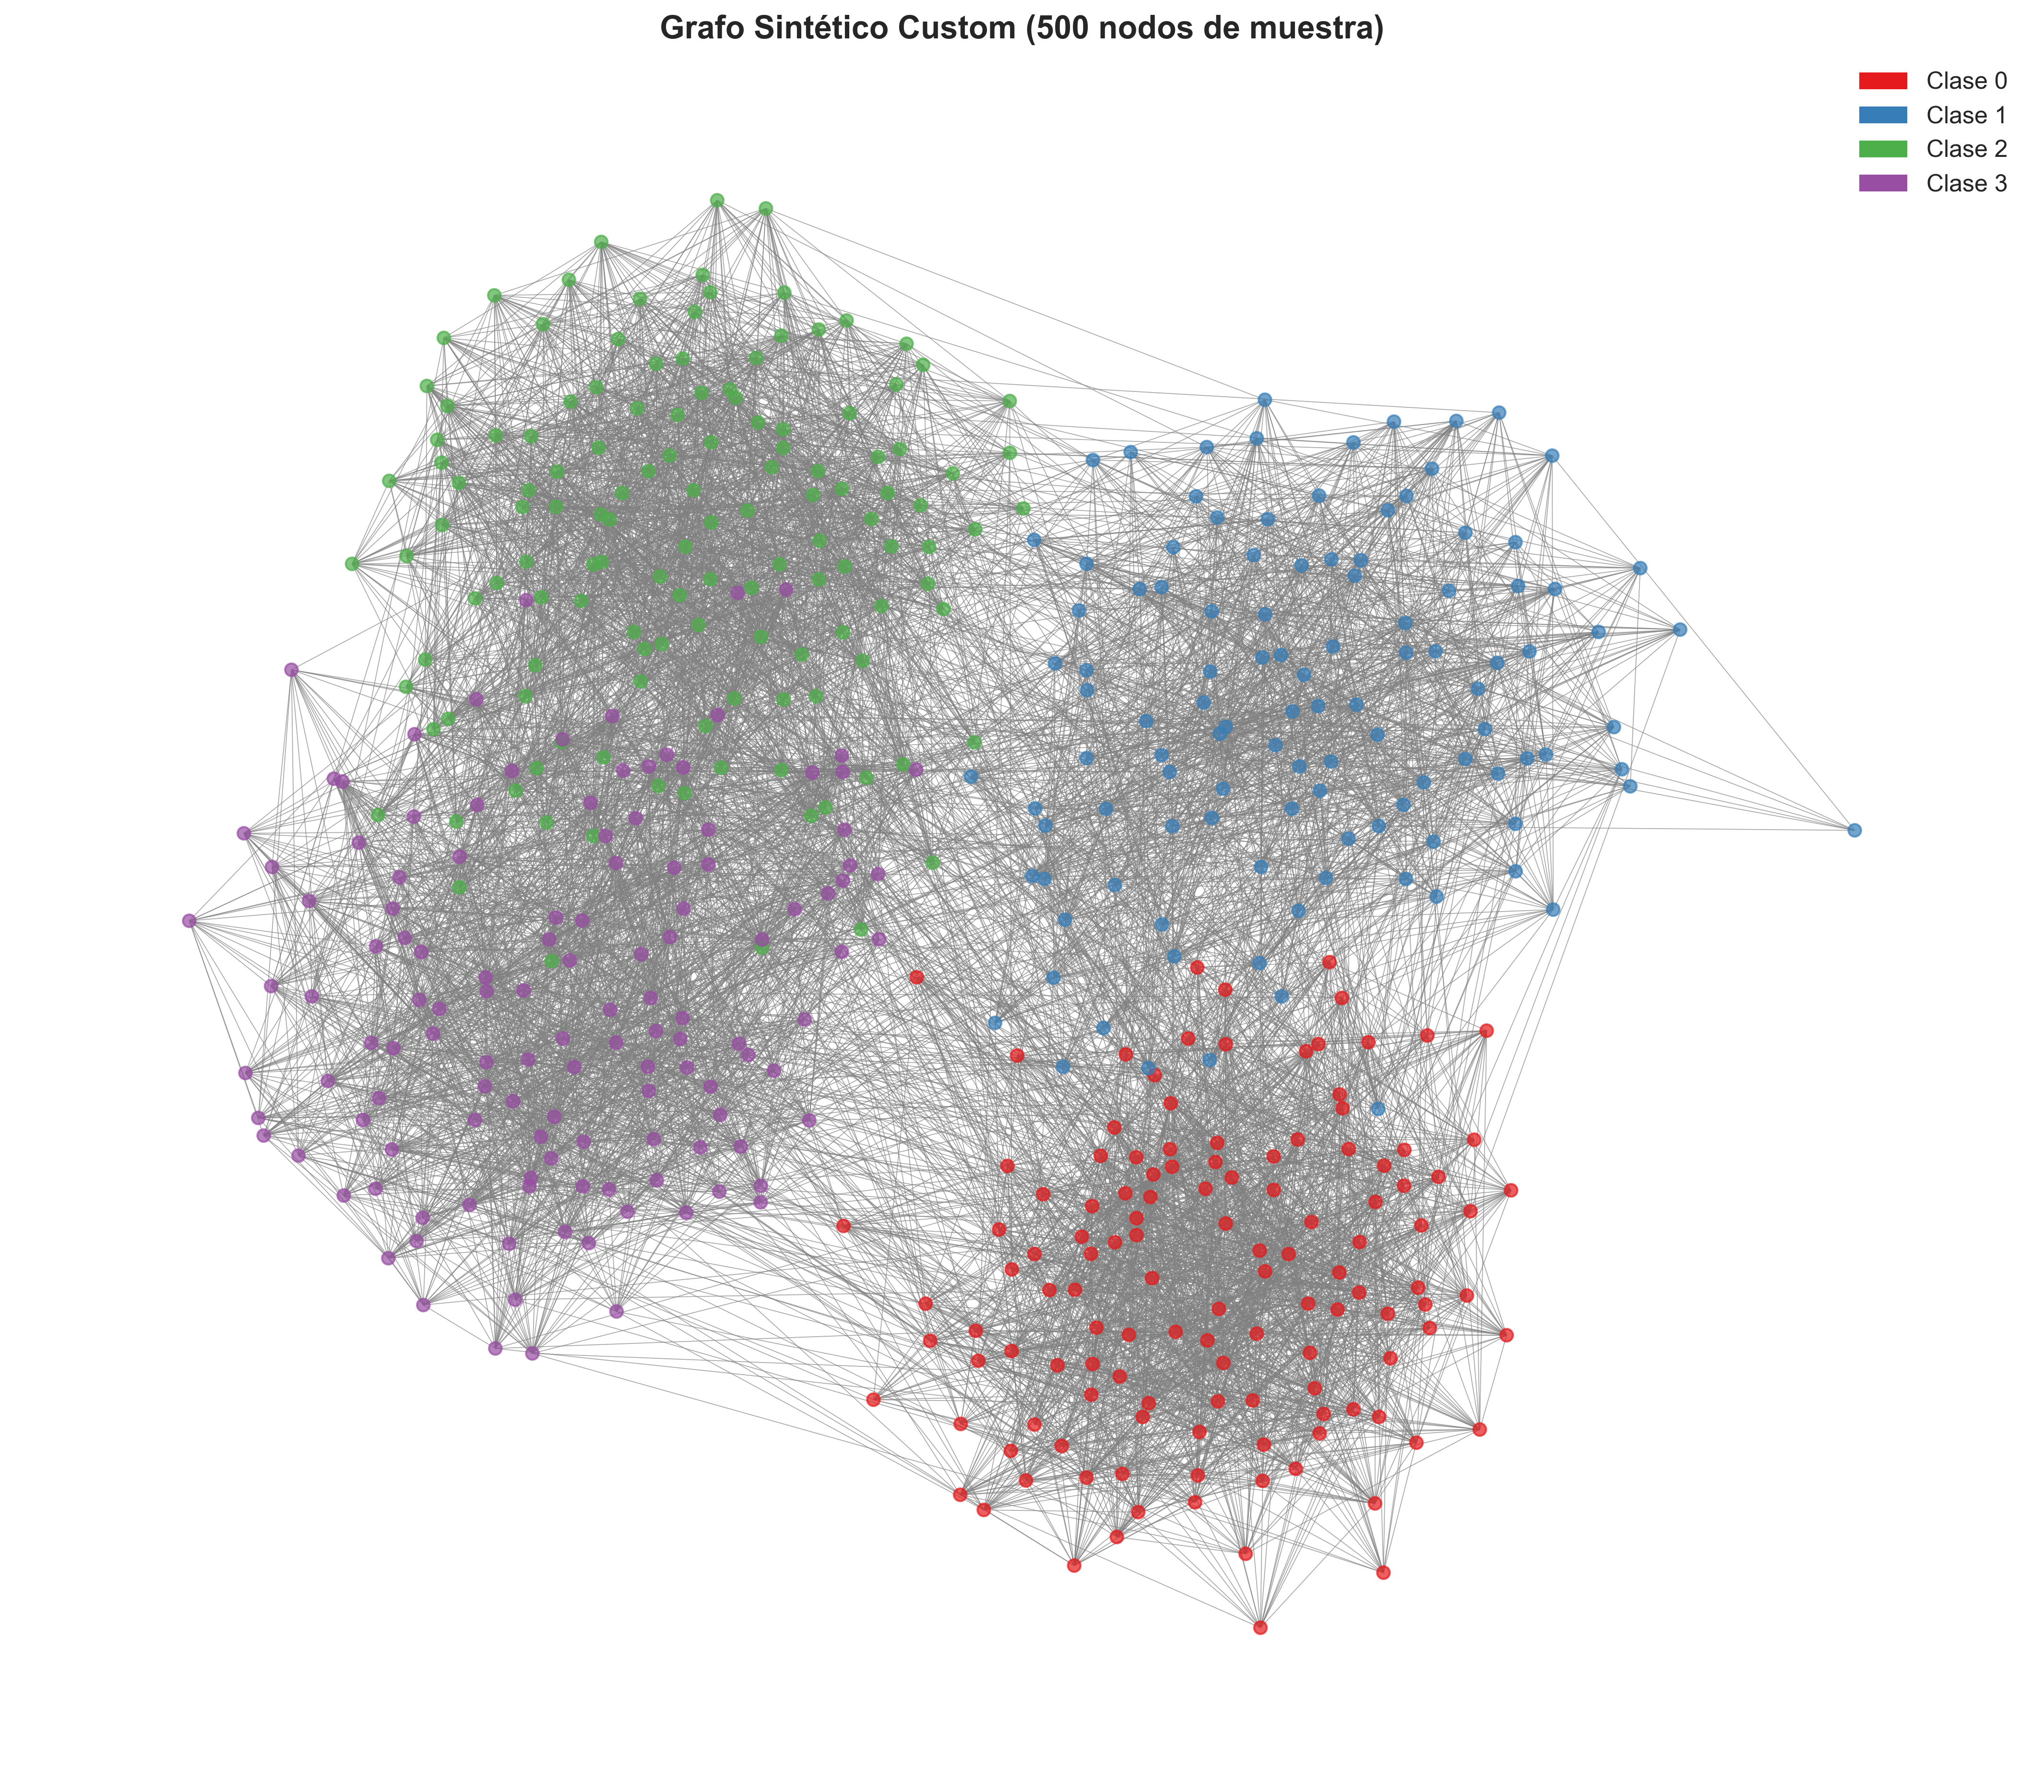
\includegraphics[width=0.8\textwidth]{images/custom_graph_structure.png}
		\caption{Visualización del grafo sintético mostrando la estructura de comunidades}
		\label{fig:graph_structure}
	\end{figure}
	
	\subsection{Modelos Implementados}
	
	\subsubsection{MLP Baseline}
	El Multi-Layer Perceptron sirve como baseline y procesa cada nodo independientemente:
	\begin{itemize}
		\item Capa 1: Linear(in\_features, hidden\_channels) + ReLU + Dropout
		\item Capa 2: Linear(hidden\_channels, num\_classes)
	\end{itemize}
	
	\textbf{Limitación}: Ignora completamente la estructura del grafo.
	
	\subsubsection{GCN}
	La Graph Convolutional Network utiliza message passing:
	\begin{itemize}
		\item Capa 1: GCNConv(in\_features, hidden\_channels) + ReLU + Dropout
		\item Capa 2: GCNConv(hidden\_channels, num\_classes)
	\end{itemize}
	
	\textbf{Ventaja}: Agrega información de vecinos, capturando la estructura del grafo.
	
	\subsection{Configuración Experimental}
	
	\subsubsection{Configuración Base}
	\begin{itemize}
		\item Hidden channels: 64
		\item Learning rate: 0.01
		\item Dropout: 0.5
		\item Weight decay: 5e-4
		\item Optimizer: Adam
		\item Epochs: 200
	\end{itemize}
	
	\subsubsection{Splits de Datos}
	Se crearon 10 splits independientes con:
	\begin{itemize}
		\item Train: 60\% (1200 nodos)
		\item Validation: 20\% (400 nodos)
		\item Test: 20\% (400 nodos)
	\end{itemize}
	
	\section{Resultados Experimentales}
	
	\subsection{Dataset Custom - Resultados Base}
	
	% NOTA: Las tablas y figuras se completarán con los resultados del notebook
	
	\begin{table}[H]
		\centering
		\caption{Resultados base en el dataset custom (media ± std sobre 10 runs)}
		\begin{tabular}{lcc}
			\toprule
			\textbf{Modelo} & \textbf{Test Accuracy} & \textbf{Mejora vs MLP} \\
			\midrule
			MLP & TODO & - \\
			GCN & TODO & TODO \\
			\bottomrule
		\end{tabular}
		\label{tab:base_results}
	\end{table}
	
	\begin{figure}[H]
		\centering
		\includegraphics[width=\textwidth]{images/custom_base_training_curves.png}
		\caption{Curvas de entrenamiento comparando MLP vs GCN}
		\label{fig:training_curves}
	\end{figure}
	
	\subsection{Análisis de Hiperparámetros}
	
	\subsubsection{Hidden Dimensions}
	Se experimentó con hidden dimensions: [16, 32, 64, 128]
	
	% TODO: Completar con resultados
	
	\subsubsection{Learning Rate}
	Se experimentó con learning rates: [0.001, 0.01, 0.1]
	
	% TODO: Completar con resultados
	
	\subsubsection{Dropout}
	Se experimentó con dropout: [0.0, 0.3, 0.5]
	
	% TODO: Completar con resultados
	
	\subsubsection{Weight Decay}
	Se experimentó con weight decay: [0, 1e-4, 5e-4]
	
	% TODO: Completar con resultados
	
	\subsubsection{Optimizers}
	Se comparó Adam vs SGD
	
	% TODO: Completar con resultados
	
	\subsection{Benchmarks: Cora y Citeseer}
	
	% TODO: Completar con resultados de benchmarks
	
	\section{Análisis y Discusión}
	
	\subsection{Performance Gap: MLP vs GCN}
	
	% TODO: Responder pregunta 1 del enunciado
	
	\subsection{Efecto de Hidden Dimensions}
	
	% TODO: Responder pregunta 2 del enunciado
	
	\subsection{Efecto de Dropout}
	
	% TODO: Responder pregunta 3 del enunciado
	
	\subsection{Análisis de Representaciones (t-SNE)}
	
	% TODO: Responder pregunta 4 del enunciado
	
	\section{Conclusiones}
	
	% TODO: Completar conclusiones
	
	\newpage
	\section{Referencias}
	
	\begin{enumerate}
		\item Kipf, T. N., \& Welling, M. (2017). Semi-Supervised Classification with Graph Convolutional Networks. ICLR.
		\item Hamilton, W. L., Ying, R.,  \& Leskovec, J. (2017). Inductive Representation Learning on Large Graphs. NeurIPS.
		\item PyTorch Geometric Documentation. \url{https://pytorch-geometric.readthedocs.io/}
	\end{enumerate}



\end{document}